\chapter{Results and Discussion}
\label{Experiments}

This chapter details the numerical processes undertaken to evaluate the performance of various GAN 
architectures. It includes model selection, structural adjustments, exploration of layer depth, and the 
impact of data augmentation on model performance. Additionally, the chapter discusses the application of 
the chosen model to a new dataset, providing insights into the practical effectiveness of the models 
in generating high-quality images. 


\section{Standard GAN Versus Other GAN Realizations}
Approximately a decade has passed since Goodfellow introduced Generative Adversarial Network (GAN), 
during which numerous variants of GAN models have been developed. For the purpose of this study, 
I have selected seven distinct GAN models for examination and minimal implementation: Standard GAN, 
Conditional GAN, Auxiliary Classifier GAN, Cycle GAN, Domain Transfer Network GAN, Coupled GAN, 
and Style GAN. Based on their foundational nature, extensive research and documentation, training and 
implementation efficiency, and flexibility and versatility, Standard GAN was selected for this study. 
The following outlines the reasons for this choice.


\begin{enumerate}
    \item Foundational Nature: Standard GAN, introduced by Ian Goodfellow et al. in 2014, serves as the 
    foundational model for all subsequent GAN variants. Understanding the principles and mechanics of 
    Standard GAN is crucial for comprehending more complex versions like Conditional GAN, Cycle GAN, 
    and Style GAN. By focusing on the Standard GAN, this study lays a solid foundation for exploring more advanced models.

    \item Widely Studied and Well-Documented: Standard GAN has been extensively researched, with a 
    vast amount of literature available. This wealth of resources provides a robust theoretical 
    background and a variety of implementation strategies, facilitating a more thorough and 
    well-supported analysis. This also means that there is ample precedent for common challenges 
    and solutions, making it easier to troubleshoot and refine the model during the study.

    \item Training and Implementation Efficiency: Compared to more complex GAN variants, 
    Standard GAN typically requires less computational power and shorter training times, 
    making it more accessible for experimentation and analysis. This efficiency allows 
    for multiple experiments and parameter tuning within the constraints of the study, 
    leading to more reliable and reproducible results.

    \item Flexibility and Versatility: Standard GAN is highly versatile and can be adapted 
    to a wide range of tasks and datasets. This flexibility makes it an excellent choice for 
    a detailed study that may involve exploring various applications or extending the model to new domains.
\end{enumerate}


\section{GAN With Convolutional or Dense Layers}

On the MNIST dataset for 3000 epochs, I compared the generated images from two GAN architectures: one using dense layers and the other using convolutional layers (CNN). It was observed that the GAN with the CNN architecture outperformed the dense layer architecture in terms of image quality, producing clearer and more realistic images.

As shown in Figures \ref{fig:gen_architecture} and \ref{fig:disc_architecture}, the generator and discriminator architectures for both dense and convolutional layers are compared. Figure \ref{fig:gen_dense} illustrates the generator with dense layers, which consists of a series of fully connected layers, while Figure \ref{fig:gen_conv} shows the generator with convolutional layers, where convolutional and transpose convolutional layers are used to capture spatial features more effectively. The same comparison applies to the discriminator architectures shown in Figure \ref{fig:disc_architecture}. The dense-layer discriminator (Figure \ref{fig:disc_dense}) is built with fully connected layers, whereas the convolutional discriminator (Figure \ref{fig:disc_conv}) leverages convolutional layers to better identify patterns in the data.

\begin{figure}[H]
    \centering
    \begin{subfigure}[b]{0.45\linewidth}
        \centering
        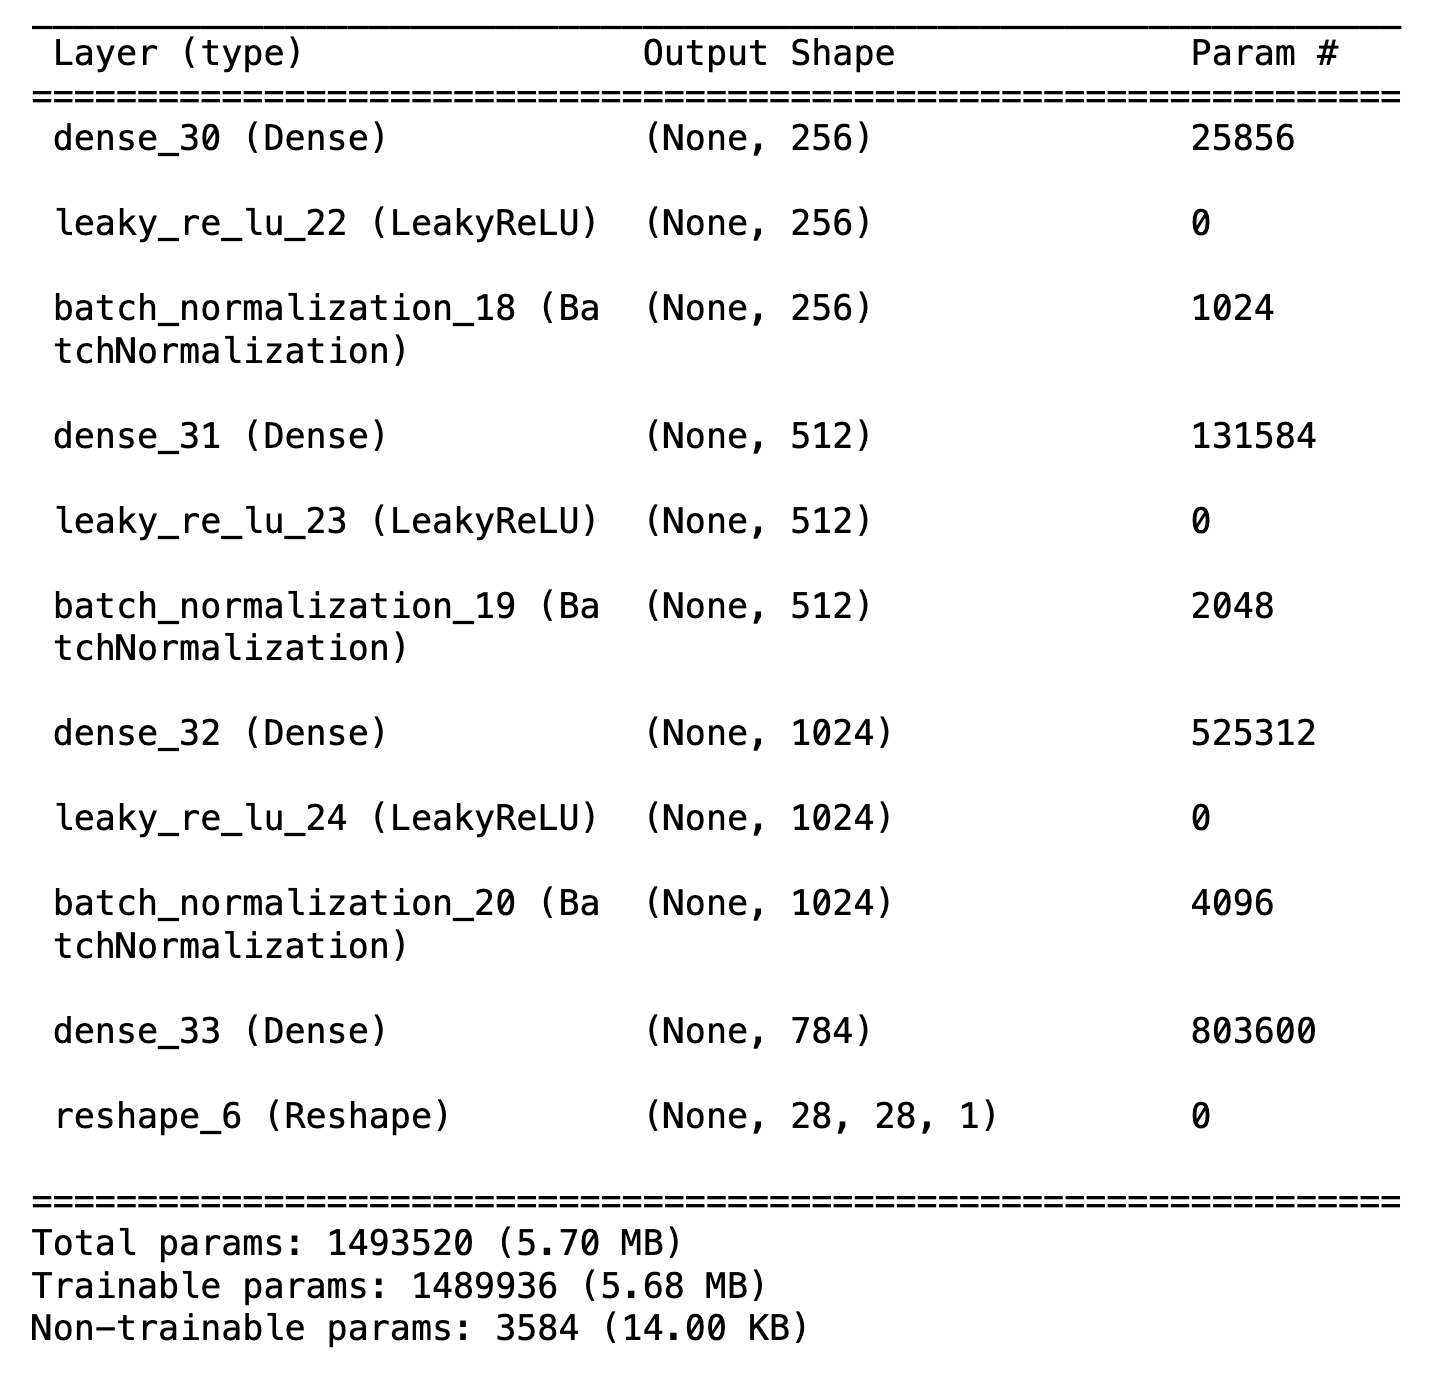
\includegraphics[width=\linewidth]{./Images/generator_dense.jpg}
        \caption{Generator with Dense Layer}
        \label{fig:gen_dense}
    \end{subfigure}
    \hspace{0.05\linewidth}
    \begin{subfigure}[b]{0.45\linewidth}
        \centering
        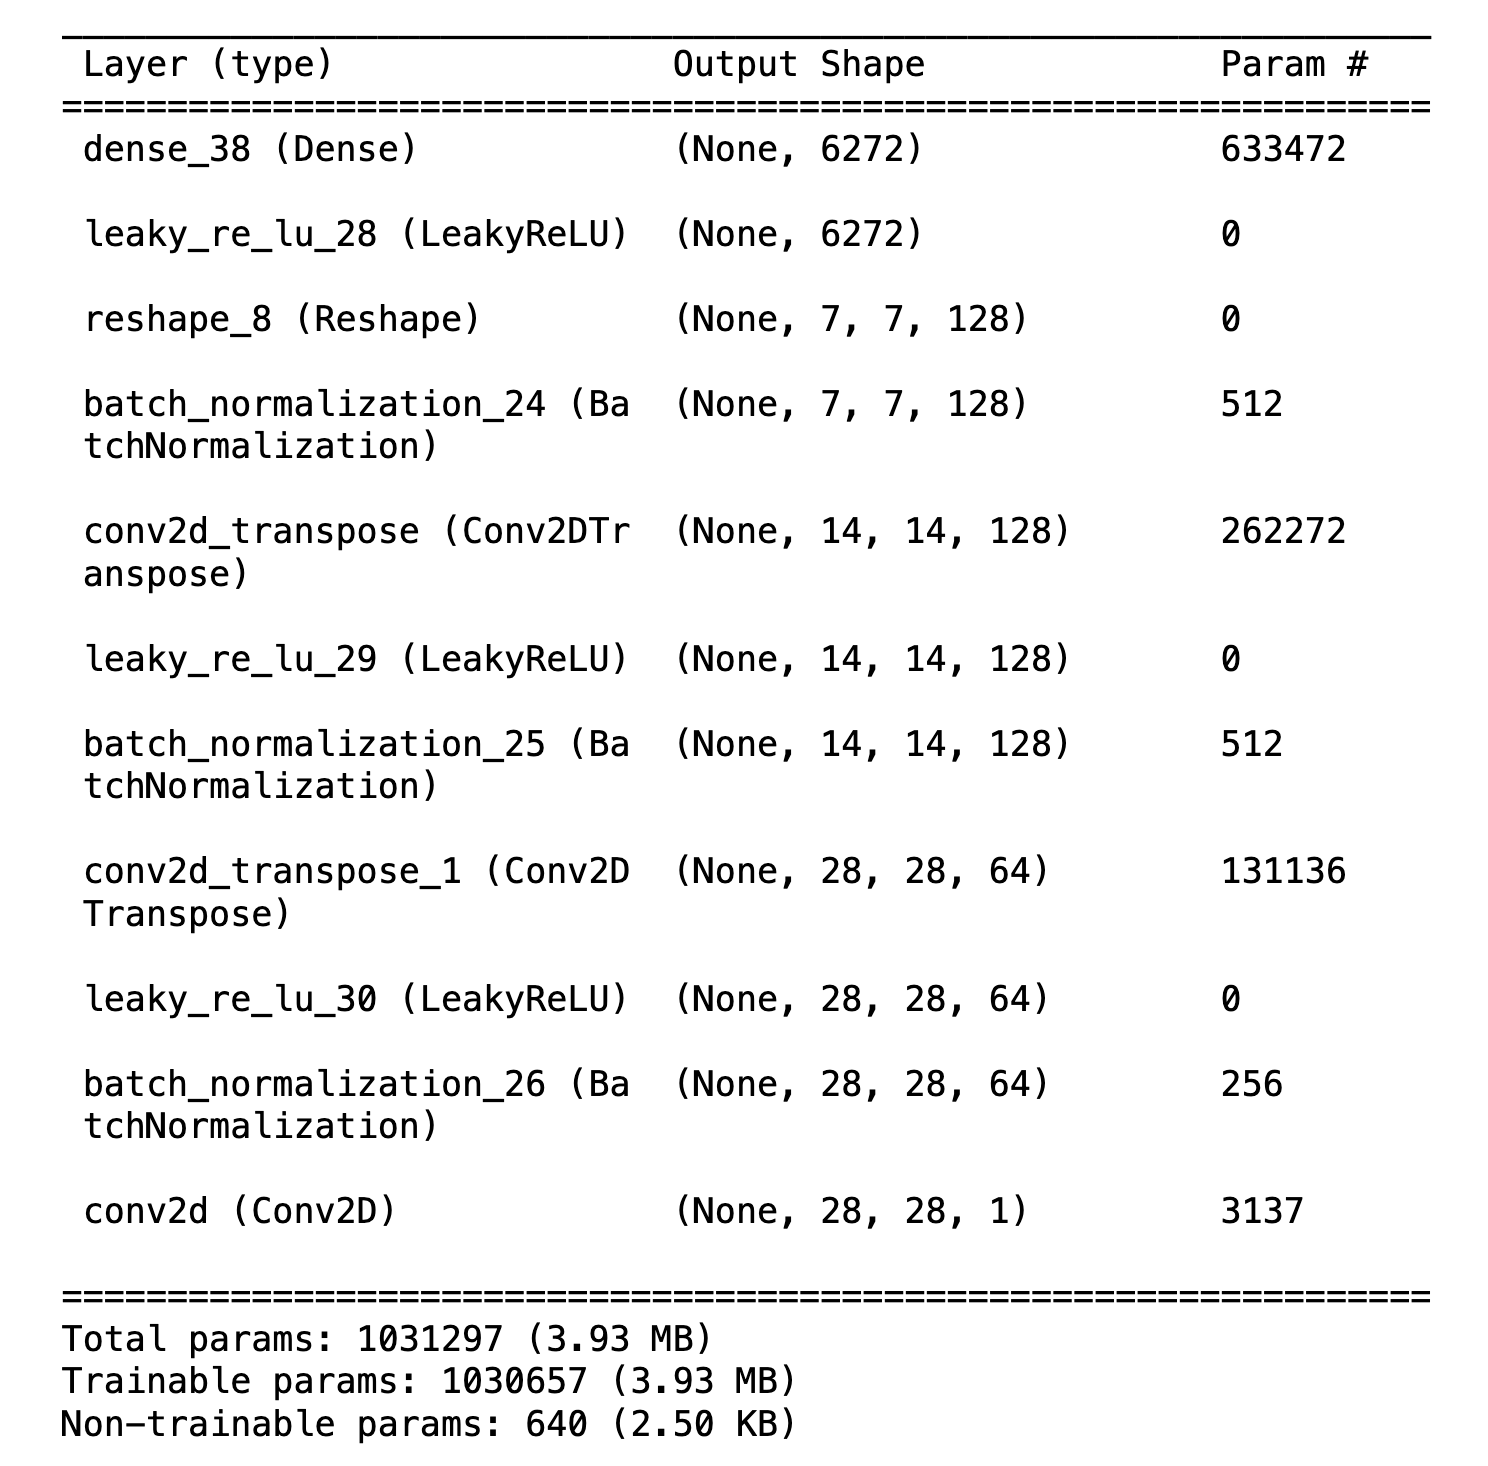
\includegraphics[width=\linewidth]{./Images/generator_cnn.jpg}
        \caption{Generator with Convolution Layer}
        \label{fig:gen_conv}
    \end{subfigure}
    \caption{Generator Architecture with Dense and Convolutional Layers}
    \label{fig:gen_architecture}
\end{figure}

\begin{figure}[H]
    \centering
    \begin{subfigure}[b]{0.45\linewidth}
        \centering
        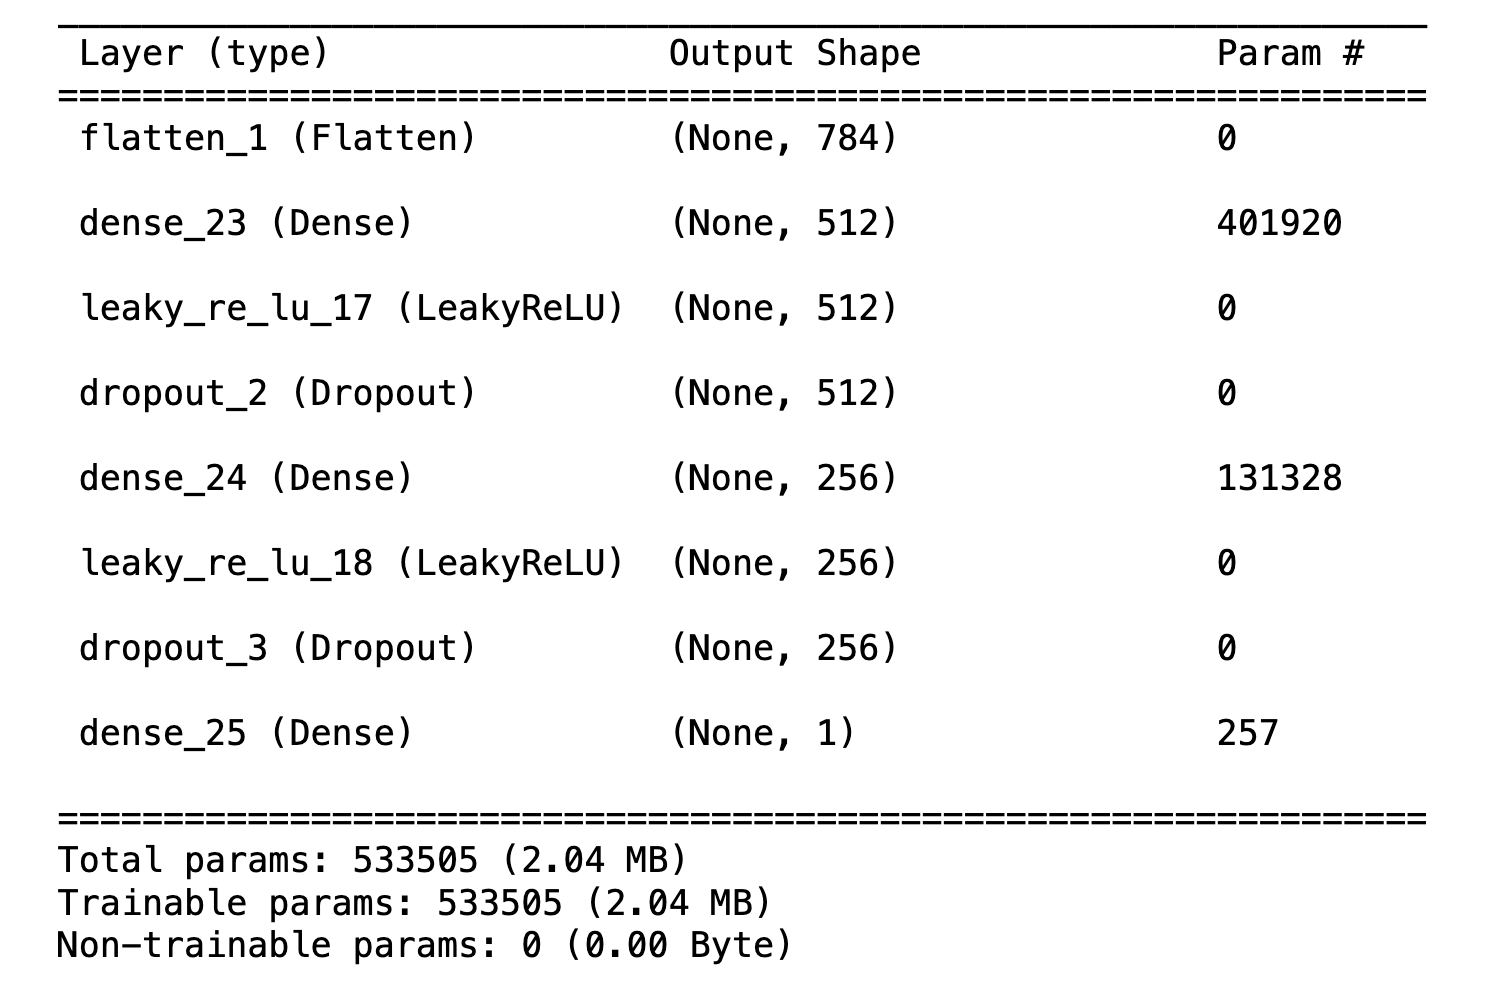
\includegraphics[width=\linewidth]{./Images/discriminator_dense.jpg}
        \caption{Discriminator with Dense Layer}
        \label{fig:disc_dense}
    \end{subfigure}
    \hspace{0.05\linewidth}
    \begin{subfigure}[b]{0.45\linewidth}
        \centering
        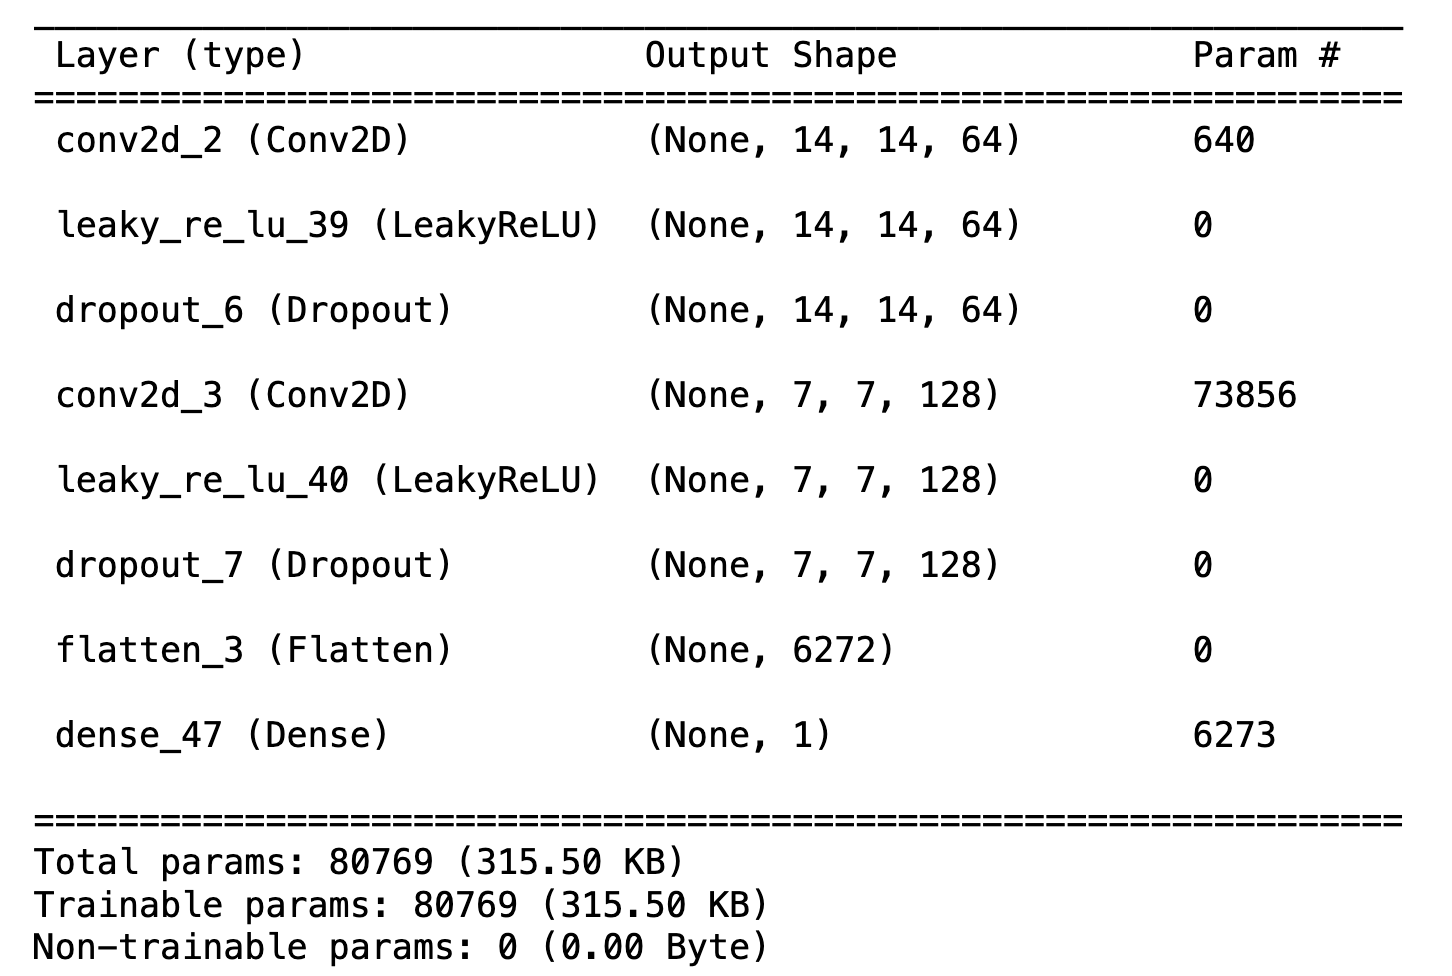
\includegraphics[width=\linewidth]{./Images/discriminator_cnn.jpg}
        \caption{Discriminator with Convolution Layer}
        \label{fig:disc_conv}
    \end{subfigure}
    \caption{Discriminator Architecture with Dense and Convolutional Layers}
    \label{fig:disc_architecture}
\end{figure}

Notably, the dense-layer models contain significantly more parameters compared to the convolutional models. The generator with dense layers has approximately 1.5 million parameters, whereas the convolutional generator has only about 1 million parameters. Similarly, the dense-layer discriminator has over 500,000 parameters, while the convolutional discriminator has only 80,000. Despite the larger parameter size, the dense-layer architectures were less effective in producing high-quality images, highlighting the advantage of convolutional layers in capturing spatial dependencies in the data.

\begin{figure}[H]
    \centering
    \begin{subfigure}[b]{\linewidth}
        \centering
        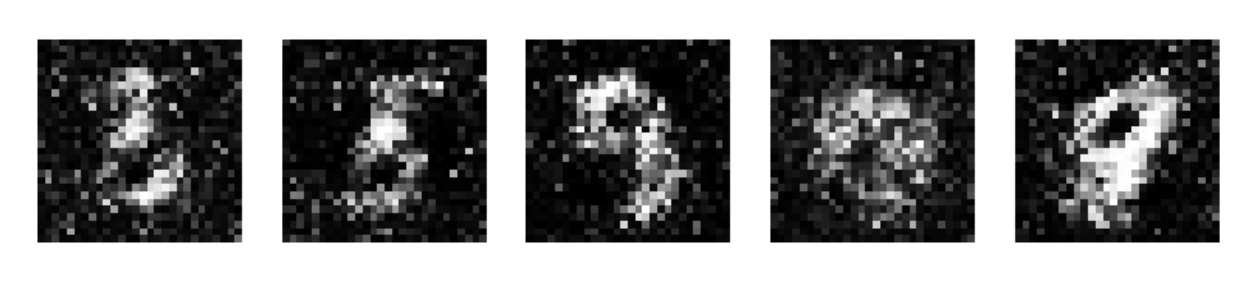
\includegraphics[width=0.7\linewidth]{./Images/generate_image_by_dense_layer.jpg}
        \caption{Images Generated by GAN with Dense Layers}
        \label{fig:generated_dense}
    \end{subfigure}
    \vspace{0.05\linewidth} 
    \begin{subfigure}[b]{\linewidth}
        \centering
        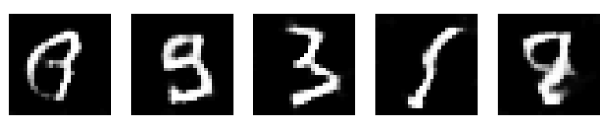
\includegraphics[width=0.7\linewidth]{./Images/generate_image_by_Convolution_layer.jpg}
        \caption{Images Generated by GAN with Convolution Layers}
        \label{fig:generated_conv}
    \end{subfigure}
    \caption{Comparison of GAN Performance at 3000 Epochs}
    \label{fig:generated_images}
\end{figure}

\begin{figure}[H]
    \centering
    \begin{subfigure}[b]{\linewidth}
        \centering
        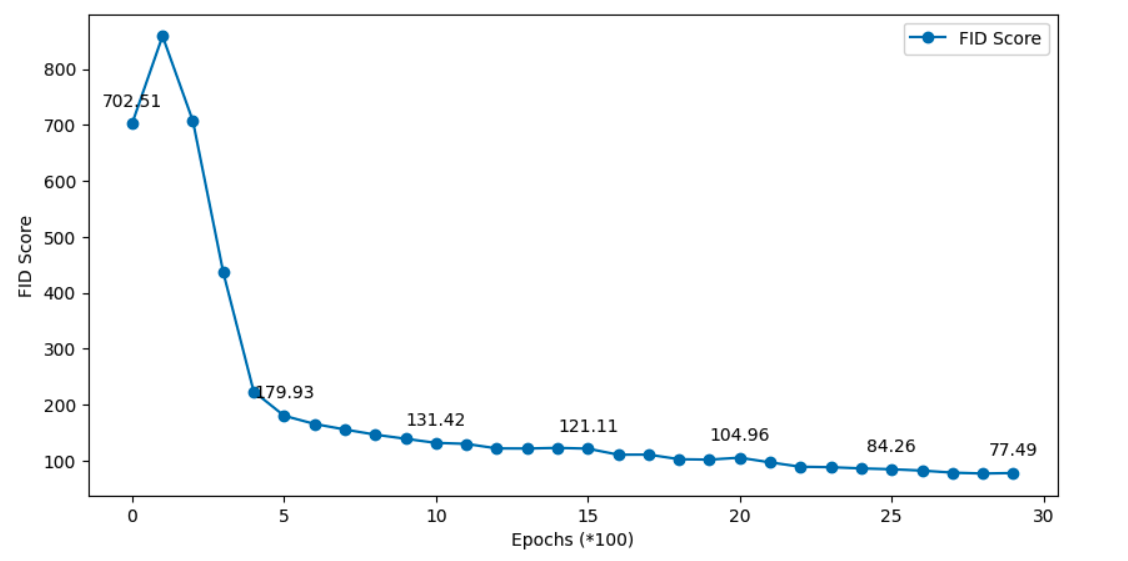
\includegraphics[width=0.7\linewidth]{./Images/fid_score_for_dense_layer.jpg}
        \caption{FID Score for Dense Layer}
        \label{fig:fid_dense}
    \end{subfigure}
    \vspace{0.05\linewidth} 
    \begin{subfigure}[b]{\linewidth}
        \centering
        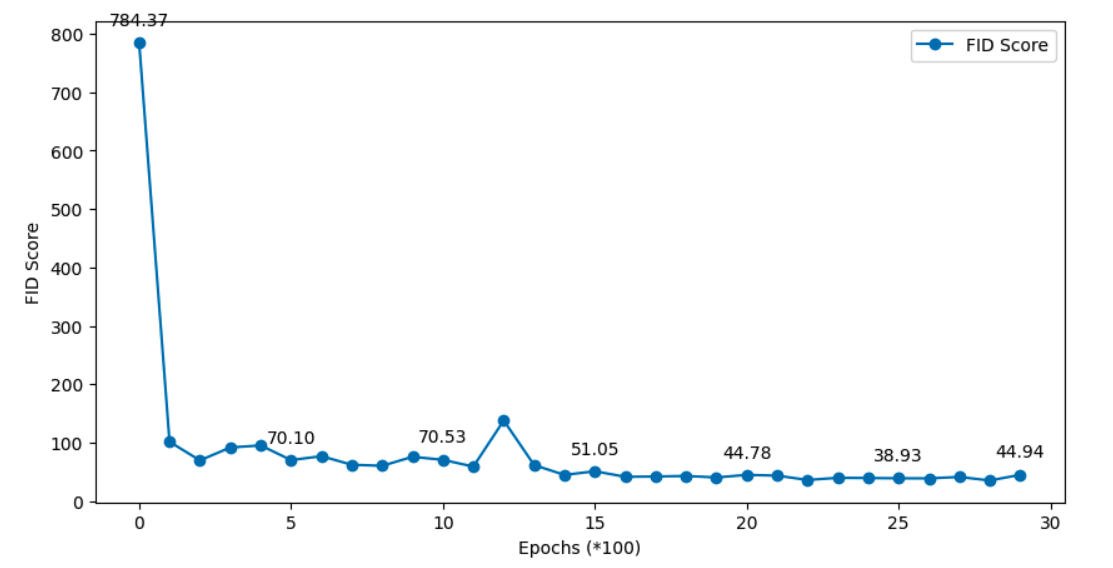
\includegraphics[width=0.7\linewidth]{./Images/fid_score_for_convolution_layer.jpg}
        \caption{FID Score for Convolutional Layer}
        \label{fig:fid_conv}
    \end{subfigure}
    \caption{FID Scores Across 3000 Epochs}
    \label{fig:fid_scores}
\end{figure}

Based on the results, the GAN model with convolutional layers demonstrated superior performance in generating high-quality images compared to the dense layer model. As shown in the generated images (Figure \ref{fig:generated_images}), the convolutional GAN produced more coherent and realistic outputs, whereas the dense layer GAN struggled to generate clear and recognizable digits. Additionally, the FID scores, which measure the dissimilarity between generated and real images, further validate this observation. The FID scores for the convolutional GAN (Figure \ref{fig:fid_conv}) are consistently lower across training epochs compared to the dense layer model (Figure \ref{fig:fid_dense}), indicating better quality in the generated images.

Given these results, I selected the standard GAN model with convolutional layers for further experiments, as it not only generated higher-quality images but also used fewer parameters, making it a more efficient and effective choice.


\section{Exploring Layer Depth}

In this section, I explored the impact of changing convolutional layers in the generator and discriminator of a GAN.

Firstly, I trained the basic convolutional GAN model three times and recorded the FID scores. Secondly, based on the basic structure, I gradually added convolutional layers to the generator, from one to three layers, while keeping the discriminator structure fixed. I trained the model three times for each configuration and recorded the FID scores, as shown in Table \ref{tab:fid_scores}.

Finally, using the base GAN with three additional convolutional layers in the generator, I gradually added convolutional layers to the discriminator, from one to three layers, while keeping the generator structure fixed. I trained the model three times for each configuration and recorded the FID scores.

\begin{table}[h!]
    \centering
    \caption{Average FID Scores for Different GAN Architectures (Lower is Better)}
    \vspace{2mm}
    \begin{tabular}{|c|c|c|c|c|}
    \hline
    \diagbox{Layers in G}{Layers in D} & \textbf{3} & \textbf{4} & \textbf{5} & \textbf{6} \\ \hline
    \textbf{3} & \cellcolor{green!50} 68.03 & 72.45 & 78.56 & 85.67 \\ \hline
    \textbf{4} & 78.95 & \cellcolor{green!50} 70.89 & 74.23 & 79.45 \\ \hline
    \textbf{5} & 99.17 & 85.36 & \cellcolor{green!50} 37.09 & 65.54 \\ \hline
    \textbf{6} & 194.66 & 71.54 & 55.21  & \cellcolor{green!50} 35.78 \\ \hline
    \end{tabular}
    \vspace{2mm}
    \caption*{\textit{Note}: A FID value below 10 is considered to represent very high-quality generated images, 
    while values between 10 and 50 indicate good quality, and values above 50 suggest average or poor quality.}
    \label{tab:fid_scores}
\end{table}

Upon comparing, I found that increasing the number of layers in either the generator or the discriminator alone worsened the model’s performance. This imbalance disrupts the dynamic equilibrium between the generator and discriminator in the GAN framework. However, simultaneously increasing the layers in both the generator and the discriminator improved the model’s performance, as demonstrated by the decreasing FID scores with higher layer counts. For example, Table \ref{tab:fid_scores} shows that increasing both the generator and discriminator layers to five results in a significantly lower FID score of 37.09 compared to the unbalanced configurations.

This finding aligns with the concept of maintaining a balance between the generator and discriminator during training, as highlighted in the literature \citep{10.48550/arxiv.1703.10717}. The importance of this balance is crucial for the effective operation of GAN, ensuring stable learning and improved image quality \citep{10.48550/arxiv.2002.02112}.    
\section{Impact of Data Augmentation on Model Performance}

The impact of various data augmentation techniques on model performance was evaluated by comparing the average FID scores across different augmentation configurations (Table \ref{tab:augmented_training_average}). The results indicate that data augmentation generally led to poorer performance in terms of image quality compared to training without any augmentation.

\begin{table}[H]
    \centering
    \caption{Average FID Scores for Different Data Augmentation Techniques}
    \begin{tabular}{|l|c|}
    \hline
    \textbf{Data Augmentation Technique} & \textbf{Average FID Score} \\ \hline
    Rotation 10° + Shifting 0.1 + Flipping & 103.49 \\ \hline
    Rotation 10° + Shifting 0.1 & 76.04 \\ \hline
    Shifting 0.1 & 70.74 \\ \hline
    Shifting 0.05 & 66.06 \\ \hline
    \rowcolor{green!25} Without Data Augmentation & 58.94 \\ \hline
    \end{tabular}
    \label{tab:augmented_training_average}
    \vspace{2mm}
    \caption*{\textit{Note}: A FID value below 10 is considered to represent very high-quality generated images, 
    while values between 10 and 50 indicate good quality, and values above 50 suggest average or poor quality.}
\end{table}

Among the techniques tested, applying a combination of rotation, shifting, and flipping resulted in the highest FID score (103.49), suggesting a significant negative impact on the generated image quality. Rotation and shifting alone slightly improved the FID score to 76.04, while reducing the shift range to 0.1 and 0.05 further improved performance, yielding FID scores of 70.74 and 66.06, respectively. The best performance was observed with no data augmentation, achieving an FID score of 58.94.

These findings suggest that, while data augmentation is commonly employed to improve model generalization, it can potentially disrupt the data distribution and hinder the optimization process when not carefully selected or overused.

\section{Applying the Model to the Animal Faces-HQ Dataset}

In this section, the Animal Faces-HQ (AFHQ) dataset was used to train a standard GAN focused on generating realistic cat images. The dataset consists of 16,130 high-quality images with a resolution of 512x512 pixels. Due to the high resolution of the original images, I downscaled them to 128x128 pixels to avoid GPU memory issues during training.

The GAN was then trained for 4000 epochs. The following results showcase the images generated by the model's generator. Figure~\ref{fig:cat_faces_generated} displays the cat faces created by the GAN.

\subsection{Model Structure and Training}

The GAN model consists of two main components: a generator and a discriminator. The generator takes a random noise vector and progressively transforms it into a full-resolution image, while the discriminator is trained to distinguish between real and generated images.

The generator architecture starts by expanding the noise vector (100 dimensions) into a 16x16x256 feature map. Several transpose convolutional layers are then used to upsample this feature map to 128x128 pixels. The discriminator processes these images using convolutional layers, which progressively downsample the input. The final output of the discriminator is a classification (real or fake).

Below is a brief summary of the generator and discriminator models:

\begin{verbatim}
def build_generator():
    model = Sequential()

    # Expand noise vector and reshape
    model.add(Dense(16*16*256, input_dim=100))
    model.add(LeakyReLU(alpha=0.2))
    model.add(Reshape((16, 16, 256)))
    model.add(BatchNormalization(momentum=0.8))

    # Upsample to 128x128
    model.add(Conv2DTranspose(256, kernel_size=4, strides=2, padding='same'))
    model.add(LeakyReLU(alpha=0.2))
    model.add(BatchNormalization(momentum=0.8))

    model.add(Conv2DTranspose(128, kernel_size=4, strides=2, padding='same'))
    model.add(LeakyReLU(alpha=0.2))
    model.add(BatchNormalization(momentum=0.8))

    model.add(Conv2DTranspose(64, kernel_size=4, strides=2, padding='same'))
    model.add(LeakyReLU(alpha=0.2))
    model.add(BatchNormalization(momentum=0.8))

    model.add(Conv2D(3, kernel_size=7, activation='tanh', padding='same'))

    return model
\end{verbatim}

The discriminator processes the generated images through a series of convolutional layers and finally classifies them as real or fake.

\begin{verbatim}
def build_discriminator():
    model = Sequential()

    model.add(Conv2D(64, kernel_size=3, strides=2, 
    input_shape=(128, 128, 3), padding='same'))
    model.add(LeakyReLU(alpha=0.2))
    model.add(Dropout(0.25))

    model.add(Conv2D(128, kernel_size=3, strides=2, padding='same'))
    model.add(LeakyReLU(alpha=0.2))
    model.add(Dropout(0.25))

    model.add(Conv2D(256, kernel_size=3, strides=2, padding='same'))
    model.add(LeakyReLU(alpha=0.2))
    model.add(Dropout(0.25))

    model.add(Conv2D(512, kernel_size=3, strides=2, padding='same'))
    model.add(LeakyReLU(alpha=0.2))
    model.add(Dropout(0.25))

    model.add(Flatten())
    model.add(Dense(1, activation='sigmoid'))

    return model
\end{verbatim}

The training was conducted over 4000 epochs with a batch size of 128. Both real and generated images were used to train the discriminator, while the generator was trained to produce images that could fool the discriminator into classifying them as real.

\begin{verbatim}
def train(generator, discriminator, gan, x_train, epochs, batch_size=128):
    valid = np.ones((batch_size, 1))
    fake = np.zeros((batch_size, 1))

    for epoch in range(epochs):
        start_time = time.time()

        # Train the discriminator
        idx = np.random.randint(0, x_train.shape[0], batch_size)
        imgs = x_train[idx]

        noise = np.random.normal(0, 1, (batch_size, 100))
        gen_imgs = generator.predict(noise)

        d_loss_real = discriminator.train_on_batch(imgs, valid)
        d_loss_fake = discriminator.train_on_batch(gen_imgs, fake)
        d_loss = 0.5 * np.add(d_loss_real, d_loss_fake)

        # Train the generator
        noise = np.random.normal(0, 1, (batch_size, 100))
        g_loss = gan.train_on_batch(noise, valid)

        end_time = time.time()
        epoch_time = end_time - start_time

        print(f"{epoch} [D loss: {d_loss[0]} | D accuracy: "
              f"{100 * d_loss[1]}] [G loss: {g_loss}] "
              f"[Epoch time: {epoch_time:.2f} seconds]")
\end{verbatim}

\subsection{Generated Results}

Figure~\ref{fig:cat_faces_generated} shows examples of the cat images generated by the GAN after training for 4000 epochs. While the model was able to capture many of the essential features of cat faces, the generated outputs still show some variation compared to the original dataset.

\begin{figure}[H]
    \centering
    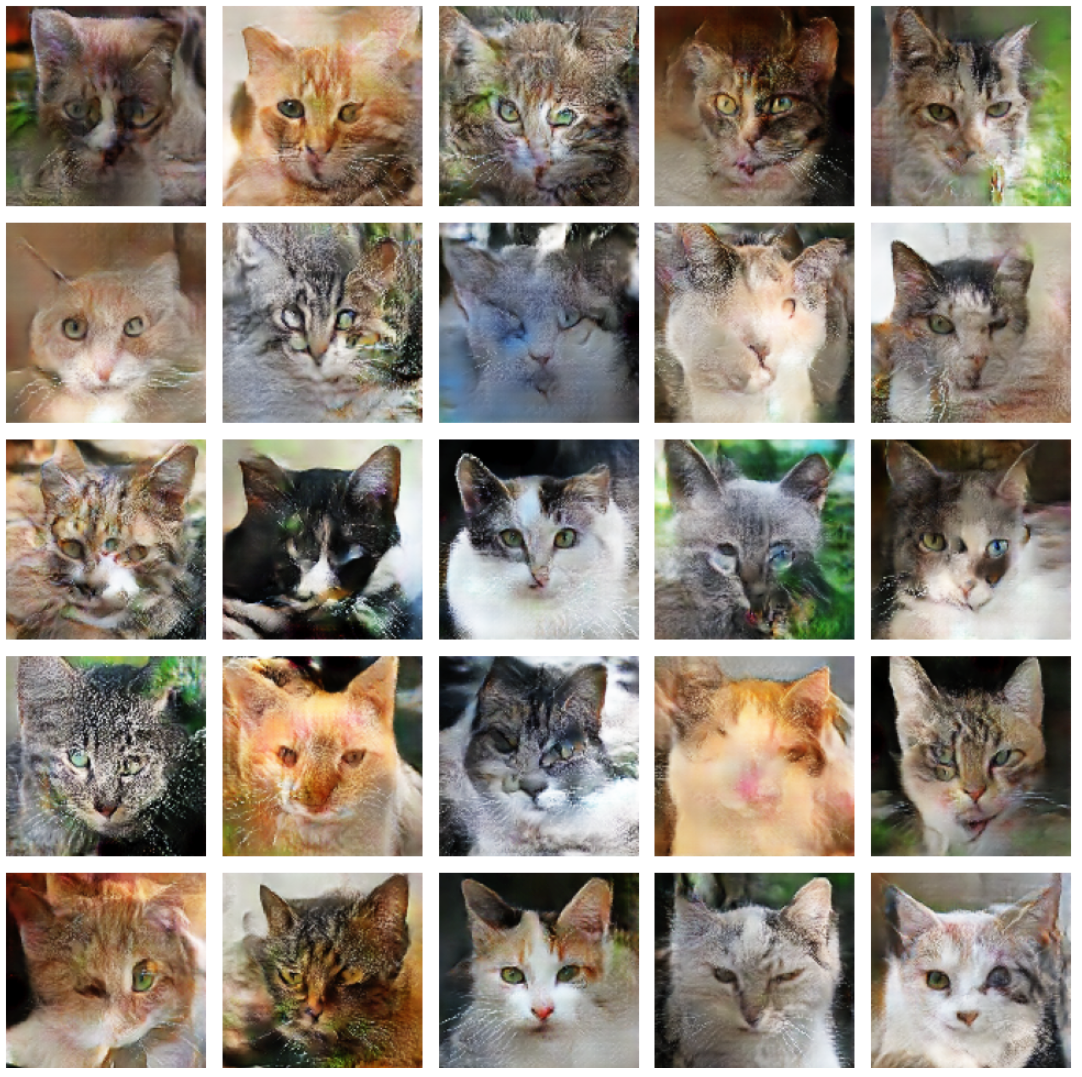
\includegraphics[width=0.8\linewidth]{./Images/apply_new_dataset.jpg}
    \caption{Cat Faces Generated by GAN}
    \label{fig:cat_faces_generated}
\end{figure}

The GAN’s architecture and training details are included in the appendix. Additionally, the full Python code for this implementation is available to provide a detailed understanding of how the model was trained and evaluated.